\chapter{Implementation}
\section{Measured Data}
	\subsection{Summary of test}
	The data used was acquired by \cite{Westhuyzen:2020} for an article assessing the charring rate of both SA-Pine and Eucalyptus.
	For the purpose of this project only the data obtained from the SA-Pine test was considered and analysed. 
	The test sample was a 100 mm by 0.9m x 0.9m panel of cross-laminated SA-pine, this sample was then divided into nine cubes of 100 mm x 100 mm x 100 mm.
	Each cube was fitted with seven Type K-thermocouples placed at consecutive 16.5 mm drilled holes.
	The test panel was tested in a furnace and was exposed to the standard ISO 834 Fire curve \ref{firecurve_fig} on one side and room temperature on the other. 
	The panel was exposed to the fire curve for 50 minutes at which stage near complete de-lamination was observed and the test ended.
	
	
	\begin{figure}[H]
	\centering 
	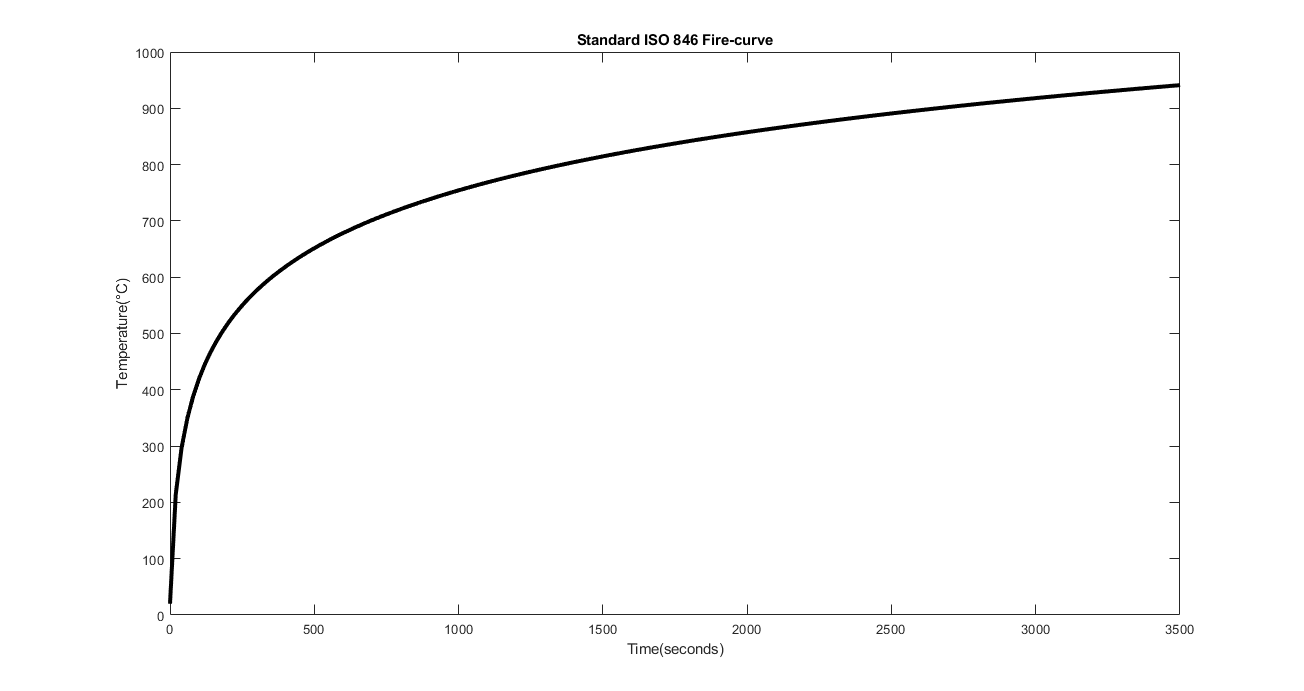
\includegraphics[width=\linewidth]{firecurve.png}
	\caption{Standard ISO fire curve TODO}
	\label{firecurve_fig}
	\end{figure}
	
	\subsection{Potential inaccuracies}
	As with most test everything is not always perfect. 
	In the data it was observed that two of the thermocouples broke during testing, this resulted in temperature with a magnitude of $10^{13}$. 
	That temperature is not possible as the highest ever recorded temperature reached was $4\text{x}10^{12}$ and that only occurred in a atomic explosion %(https://www.insidescience.org/news/hottest-temperature-universe-measured)% 
	This malfunction required that two of the depth measurements were no longer the average between nine samples but instead the average between eight.
	
	Another inaccuracy that could potentially influence the accuracy of the final result is the accuracy of the depth of the holes in which the thermocouples were placed. 
	As this was done by hand. %in the laboratory.
	
	There is also debate about the significance of the contribution of the timber burning to the temperature inside the furnace. 
	For the purposes of this project it will be assumed that the timber burning does not contribute to the temperature inside the furnace.
	
	The assumption that the panel is constantly at room temperature on the outside is also inaccurate as there is heat radiating from the panel that increases the temperature surrounding the panel.

\subsubsection{Results}

\begin{figure}[H]
	\label{measured_fig}
	\centering
	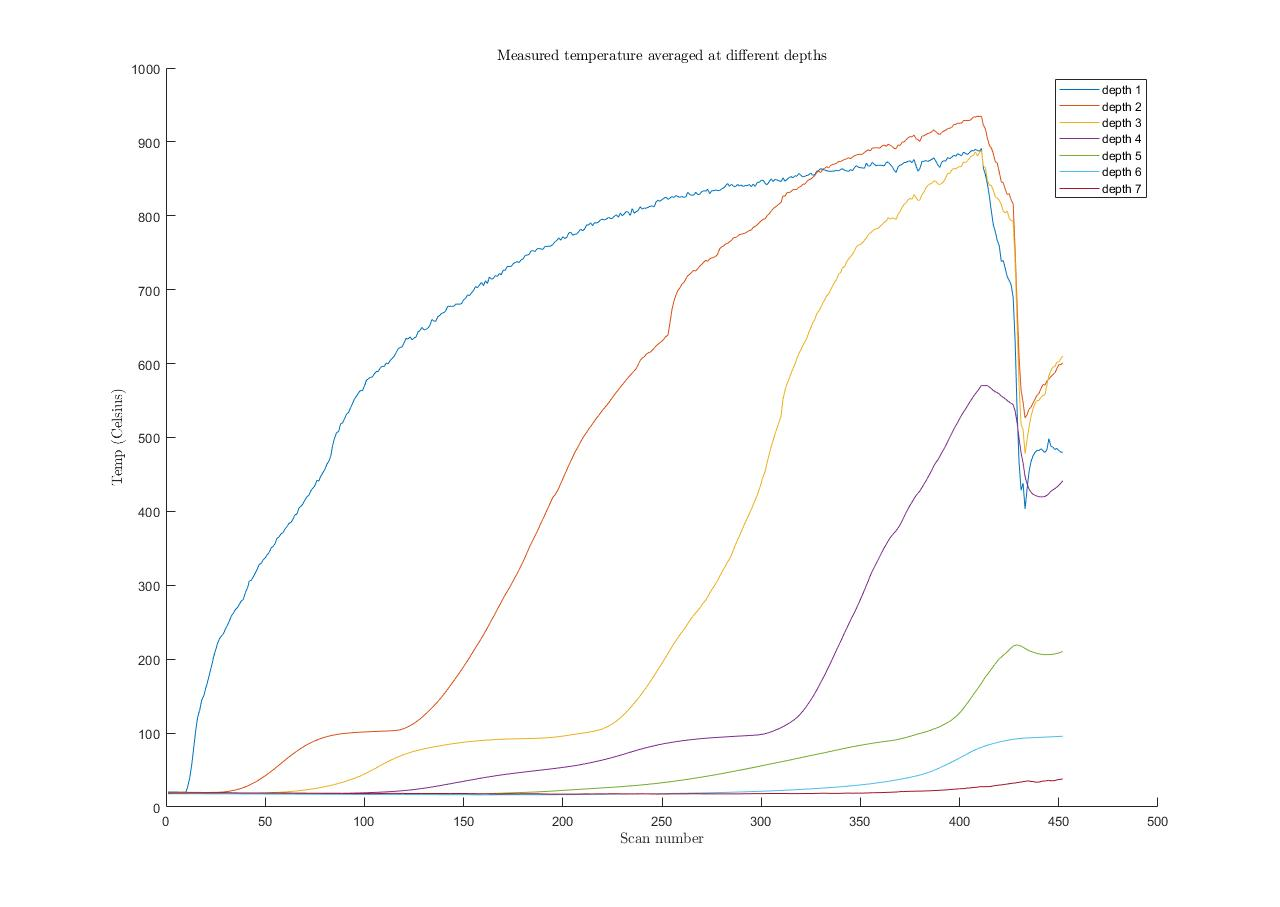
\includegraphics[width=5.5in,]{measured_data.jpg}
\end{figure}


\section{Inversion method}
%here we will discuss everything that we did